\section{Evaluation}
\label{sec:evaluation}

In this section, we present the evaluation of WiGEM on the two different testbeds. 
As a part of the evaluation, we determine the number of power levels ($K$) that should 
be used for the modeling. Our test cases include heterogeneous devices as described before with unmodeled hardware and power level characteristics, this providing a very realistic
benchmarking. We also compare WiGEM with respect 
to a simple propagation model based scheme (that also requires no pre-deployment effort) as well as well-known, high-performing schemes such as RADAR and Probabilistic~\cite{Haeberlen:2004:PRL:1023720.1023728,Youssef:2008:HLD:1399551.1399558,Roos} (they require significant pre-deployment effort, but provide the best accuracy). In addition we evaluate how the size
of the learning data set or mobility impacts the accuracy of WiGEM. 

%we present a comprehensive overview of our experimental results. We evaluate the performance of WiGEM on our two experimental testbeds. We attempt to answer the following questions.
%
%\begin{itemize}
%
%\item What is the number of power-levels that we should use in WiGMM i.e what is the value of K (mentioned in Section \ref{subsec:latentvariablesfortargetlocationsandpowerlevels} above) that we should use when we run WiGEM on the back end localization server ? 
%\item How does the WiGEM localization accuracy vary as the size of the learning data-set increases ?
%\item What is the WiGEM accuracy for heterogenous devices with unmodelled hardware and power-level characteristics ?
%\item How does WiGEM perform with respect to a model-based scheme that uses the indoor radio path loss propagation model ? This presents a true head-to-head comparison because neither needs pre-deployment effort and can work on the same granularity of discretization of the target space.
%\item How does WiGEM perform with respect to schemes that build RF signal maps like RADAR and Probabilistic \cite{Haeberlen:2004:PRL:1023720.1023728, Youssef:2008:HLD:1399551.1399558, Roos} . This experiment shows how the WiFi hardware variance problem can impact the accuracy of RF signal map schemes and also show the impact of training granularity for signal map based schemes.
%\item Can the mobility of a client can actually improve WiGEM's localization accuracy ?
%
%\end{itemize}


All reported experiments with WiGEM uses half of the measured data set at each location for learning and the other half for testing and validation. The learning part reflects the 
typical learning process for WiGEM.
The general idea is that a typical client device will naturally transmit multiple (likely many) packets for its own network use. It can always be forced to transmit some number of packets for use in localization if it does not naturally transmit anything. The sniffed RSSI vectors for these packets will form the learning set to be used in WiGEM localization. The client does not need to be stationary and is free to move about while the learning set is gathered. Two important questions now are the determination of a suitable number of power levels ($K$) to use for the learning and the size of learning set. These are addressed next.  

%As mentioned in Section \ref{subsec:datacollectionmethodology} above, the CEWIT testbed has 45 distinct locations and CSD has 27 distinct locations, and for each distinct location on the map and for each device type we have a set of 200 RSS tuples. 
%We divide these 200 tuples into two sets of 100 tuples each: one for learning the WiGMM parameters and the other for testing the WiGEM localization results. Each device type is considered separately. 
%

\subsection{Number of Powers Levels and Learning Set Size}
\label{subsec:numberofpowerlevelstouseingem}

Figure \ref{fig:powerlevelsvserrordistance} shows the results of the average error distance (in meters) for the four devices across  varying number of power levels used in WiGEM. We see that the average error distance hits a plateau after K = 31. This is an interesting result because it helps us bound the number of power levels to use. We use a value of K = 45 in the subsequent experiments. 

%\subsection{Localization accuracy in WiGEM as a function of the learning set size.}
%\label{subsec:localizationaccuracyasafunctionofthelearningsetsizeingem}
%
\begin{figure}[h!]
\centering
  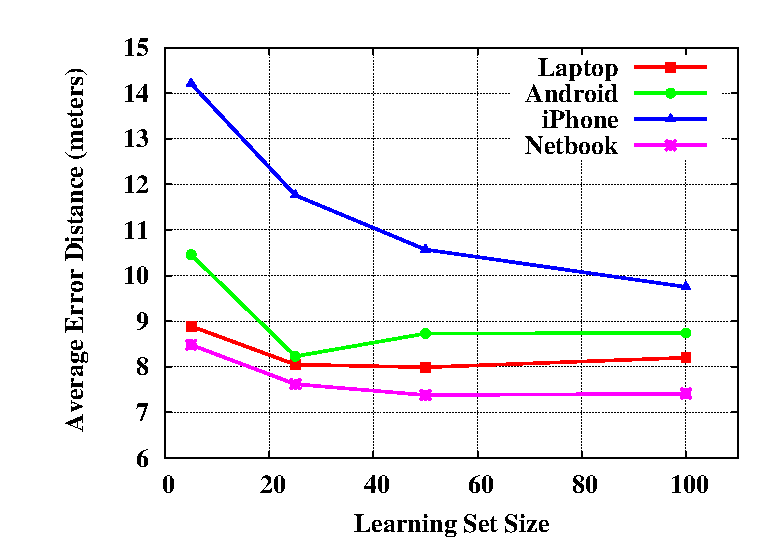
\epsfig{file=Figs4Paper/CEWIT/LearningSize4Paper_CEWIT/LearningSetSize_cewit.eps, height=1.5in, width=2.5in}
  \caption{Average error distance results for WiGEM
   as a function of the learning set size (CEWIT testbed).}
  \label{fig:learningsetsizevserrordistance}
\end{figure}

Having fixed the number of power levels to use, we now study how the size of the learning data-set changes the average error distance. Recall here that as part of our data collection methodology, we have 200 RSS tuples for every location on the map for each of the four device types. This time we again divide the 200 tuples into two sets: one set for learning and the other for testing. The test set size is kept fixed at 100 RSS tuples. From the remaining tuples, the learning set size is varied from 2 tuples going up to 100 tuples. Figure~\ref{fig:learningsetsizevserrordistance} shows the results of the average error distance (in meters) in the CEWIT testbed as the size of the learning set varies. We observe that for all the four devices, the average error does not vary much as we move from 50 training samples to 100 training samples. The CSD testbed results (not included here) converged after 25 samples itself. The experiments that follow have been done keeping the WiGEM learning set size at 100 and using the remaining 100 samples for testing the localization accuracy.  

\subsection{WiGEM Accuracy With Heterogeneous Devices}
\label{subsec:gemaccuracyforheterogeneousdevices}

\begin{figure*}
	\centering
	      \subfloat[CEWIT testbed]{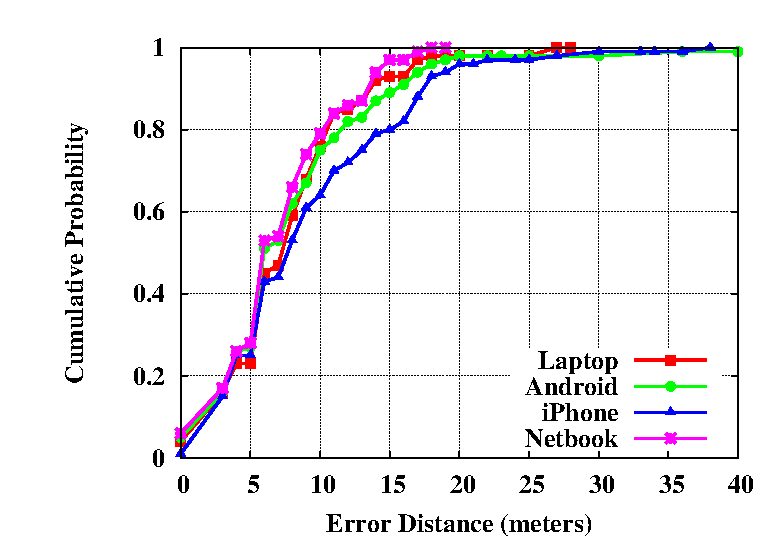
\includegraphics[height=1.5in, width=2.5in]{Figs4Paper/CEWIT/Gem4Devices_CEWIT/4Devices_cewit.eps}}
	      \subfloat[CSD testbed]{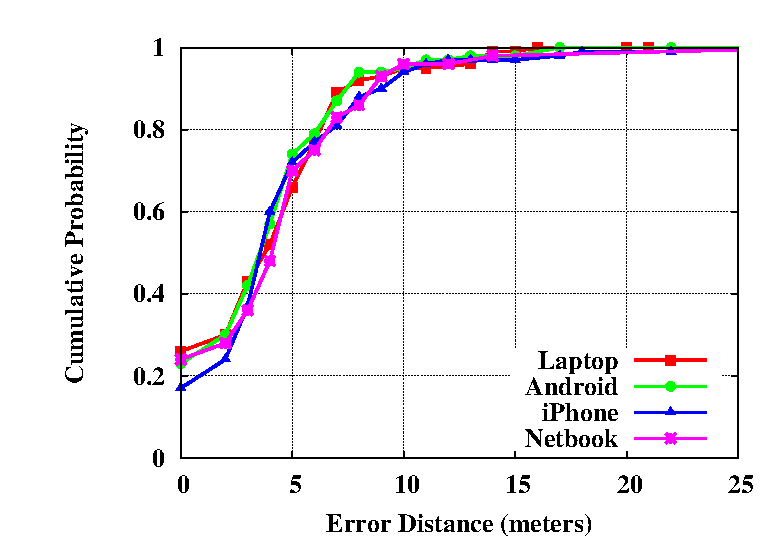
\includegraphics[height=1.5in, width=2.5in]{Figs4Paper/CSD/Gem4Devices_CSD/4Devices_csd.eps}}
	\caption{CDF of WiGEM's location accuracy for multiple devices.}
	\label{fig:gemheterogeneousdevices}
\end{figure*}

Figure \ref{fig:gemheterogeneousdevices} plots CDFs of error distances to show how WiGEM performed across the four test devices (Section \ref{subsubsec:testdevices}) on both the testbeds. For both the testbeds, the accuracy estimates are pretty similar for all the devices. Thus, we see that WiGEM can adapt itself for heterogeneous devices that possibly work at different transmit power levels. In Section \ref{subsec:comparisonswithschemesthatuserfsignalmaps} below, we show how RF-signal map based techniques show substantial degradation in accuracy owing to such hardware variations. 

\subsection{Baseline Comparison with a Model-based Scheme}
\label{subsec:baselinecomparisonwithamodelbasedscheme}

\begin{figure*}
	\centering
	      \subfloat[CEWIT testbed]{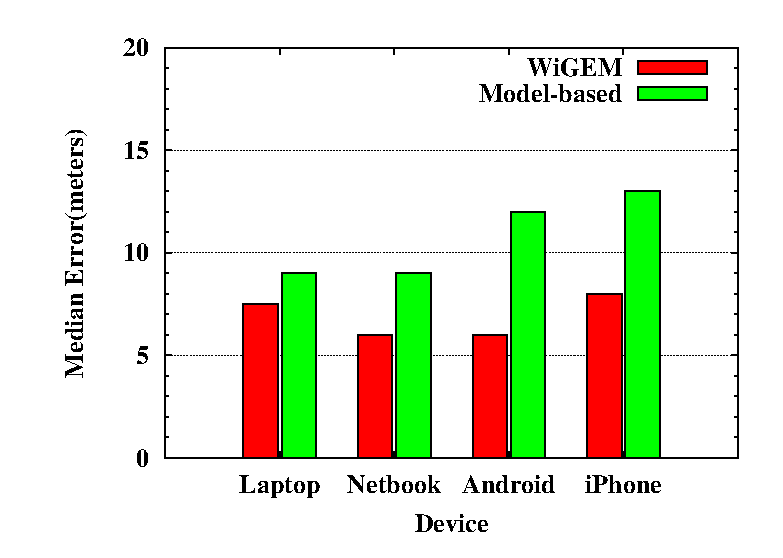
\includegraphics[height=1.5in, width=2.5in]{Figs4Paper/CEWIT/Baseline4Paper_CEWIT/BaselineComparisonsMedianError_cewit.eps}}
	      \subfloat[CSD testbed]{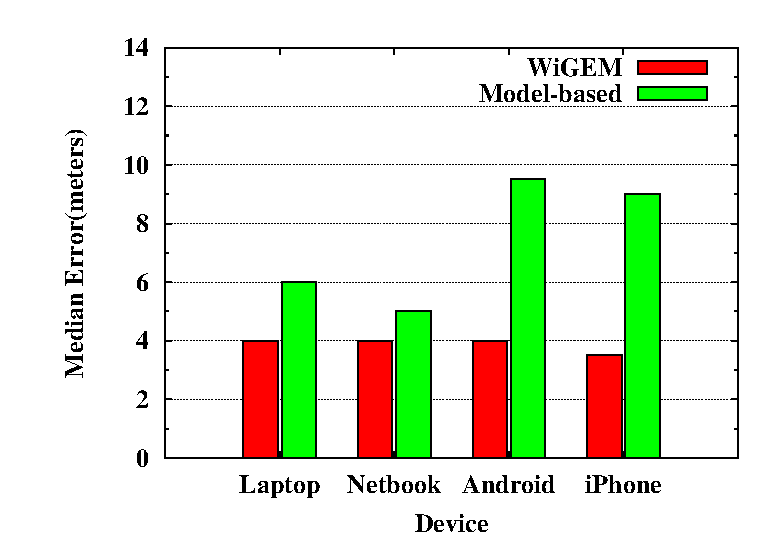
\includegraphics[height=1.5in, width=2.5in]
	      {Figs4Paper/CSD/Baseline4Paper_CSD/BaselineComparisonsMedianError_csd.eps}}
	\caption{Baseline Comparisons.}
	\label{fig:baselinecomparisons}
\end{figure*}

% \begin{figure*}
% \begin{minipage}{0.5\textwidth}
% 	{\centering
% 	  \subfloat[Probabilistic]{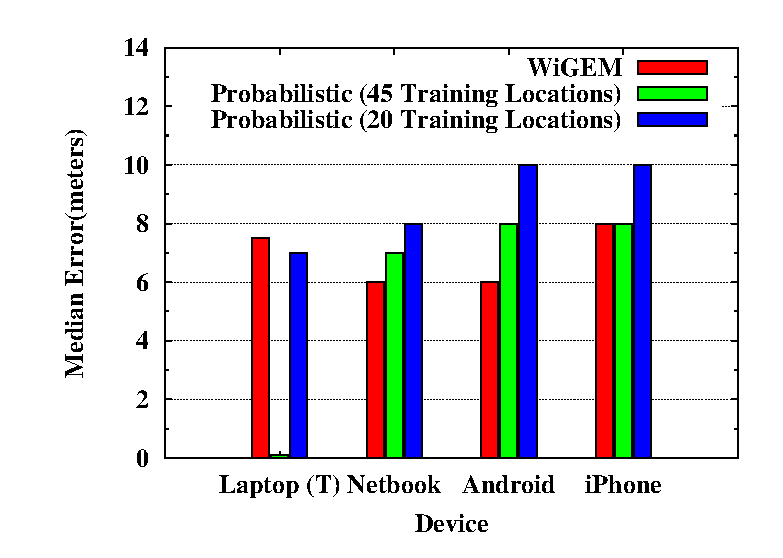
\includegraphics[width=0.5\textwidth]{Figs4Paper/CEWIT/HRComparisons4Paper_CEWIT/HRComparisonsMedianError_Probabilistic_cewit.eps}}
% 	  \subfloat[RADAR]{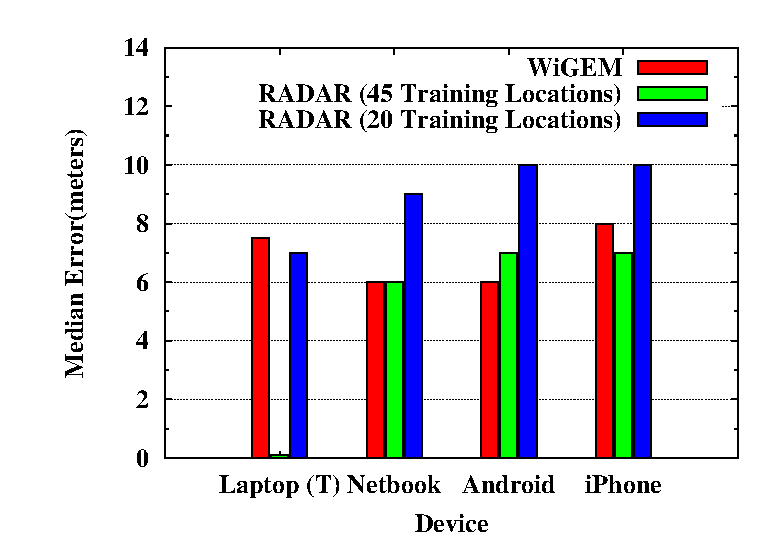
\includegraphics[width=0.5\textwidth]{Figs4Paper/CEWIT/HRComparisons4Paper_CEWIT/HRComparisonsMedianError_RADAR_cewit.eps}}
% 	\caption{Comparisons on the CEWIT Testbed}
% 	\label{fig:HR_on_cewittestbed}
% 	}
% \end{minipage}\quad
% \begin{minipage}{0.5\textwidth}
% 	{\centering
% 		\subfloat[Probabilistic]{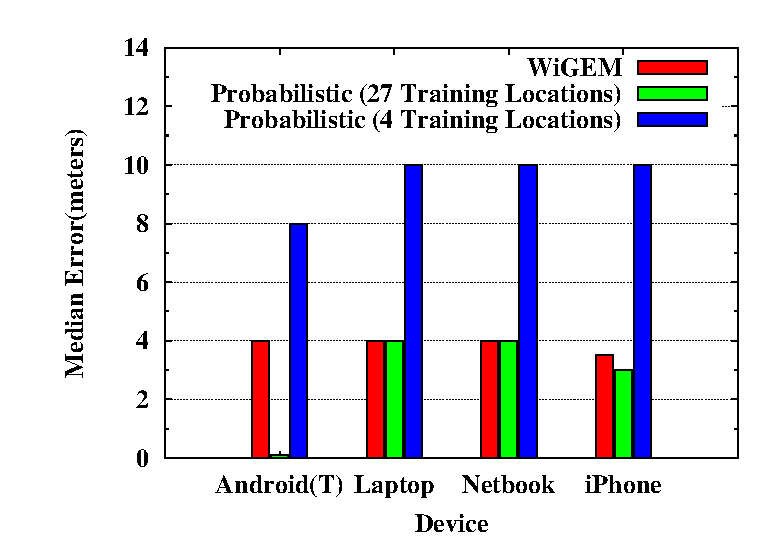
\includegraphics[width=0.5\textwidth]{Figs4Paper/CSD/HRComparisons4Paper_CSD/HRComparisonsMedianError_Probabilistic_csd.eps}}
% 		\subfloat[RADAR]{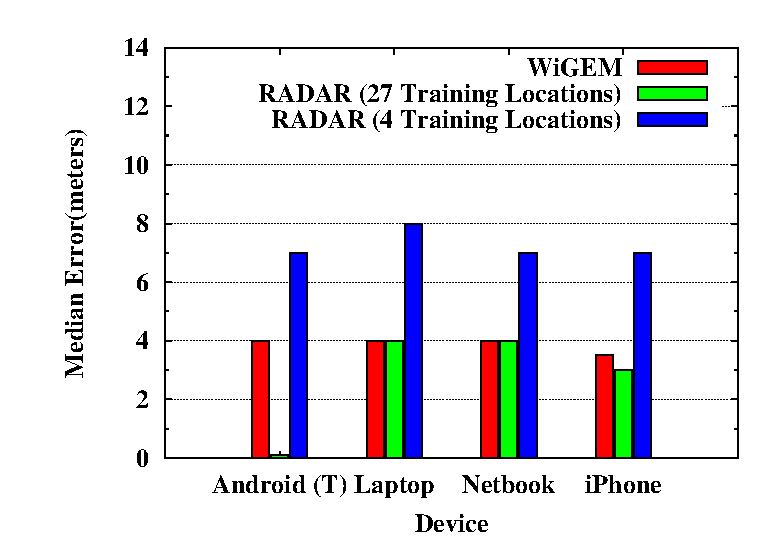
\includegraphics[width=0.5\textwidth]{Figs4Paper/CSD/HRComparisons4Paper_CSD/HRComparisonsMedianError_RADAR_csd.eps}}
% 	\caption{Comparisons on the CSD Testbed}
% 	\label{fig:HR_on_csdtestbed}
% 	}
% \end{minipage}
% \end{figure*}

Now we analyze the performance of WiGEM with respect to a model-based scheme that uses the indoor radio propagation model (Section~\ref{subsec:handlingidentifiabilityinourmodel}). 
Neither of the techniques need pre-deployment effort. We want to basically establish that
the learning technique used in WiGEM is buying us something relative to a generic radio
propagation model. 
% Both our testbeds, CEWIT and CSD, have been discretized as shown in Figure \ref{fig:experimenttestbed}. There are 267 grid vertices inside the CEWIT testbed roughly every 2.75 meters. The CSD testbed has 36 grid vertices roughly every 3.1 meters. WiGEM can localize a given target RSS vector to any of these grid vertices. As mentioned in Section \ref{subsec:datacollectionmethodology}, the data for our experimental evaluation is coming from 45 distinct locations on the CEWIT testbed and 27 distinct locations in the CSD testbed. There are 200 RSS tuples for every location on the map for each of the four device types. As mentioned above in Section \ref{subsec:localizationaccuracyasafunctionofthelearningsetsizeingem}, WiGEM is using a learning set size of 100 RSS samples with 45 power levels to build the WiGMM model. Thus the test-set for both the algorithms is remaining 100 RSS tuples from each location. Each device type is evaluated separately.

The log-distance path loss mentioned in Section~\ref{subsec:handlingidentifiabilityinourmodel} is used to estimate the RSS that should be observed at a sniffer for each grid vertex inside the target space. These RSS values are used to initialize WiGEM, as mentioned in Section~\ref{subsec:handlingidentifiabilityinourmodel}. The model-based algorithm also uses these same RSS values with a suitable metric to give a final location estimate. Similar to \cite{Bahl00radar:an}, the model-based algorithm that we use here uses the `nearest neighbor in signal space' as the metric of choice. 
Figure~\ref{fig:baselinecomparisons} shows the median error for both techniques. Note that WiGEM performs better than the model-based scheme across all device types in both testbeds. The performance improvement is quite substantial for the phone-based devices -- with the median error distance reducing to roughly half. 

\subsection{Comparison with Schemes Using RF Signal Maps}
\label{subsec:comparisonswithschemesthatuserfsignalmaps}

\begin{figure*}
	\centering
	      \subfloat[WiGEM vs. Probabilistic]{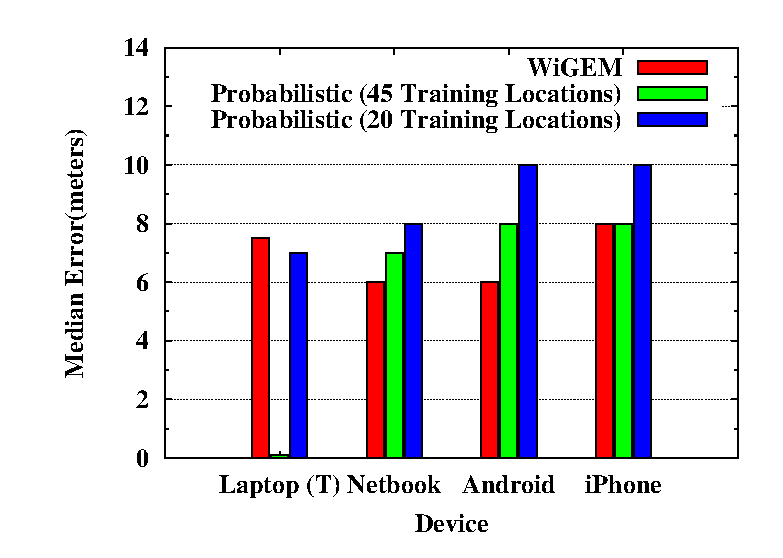
\includegraphics[height=1.5in, width=2.5in]{Figs4Paper/CEWIT/HRComparisons4Paper_CEWIT/HRComparisonsMedianError_Probabilistic_cewit.eps}}
	      \subfloat[WiGEM vs. RADAR]{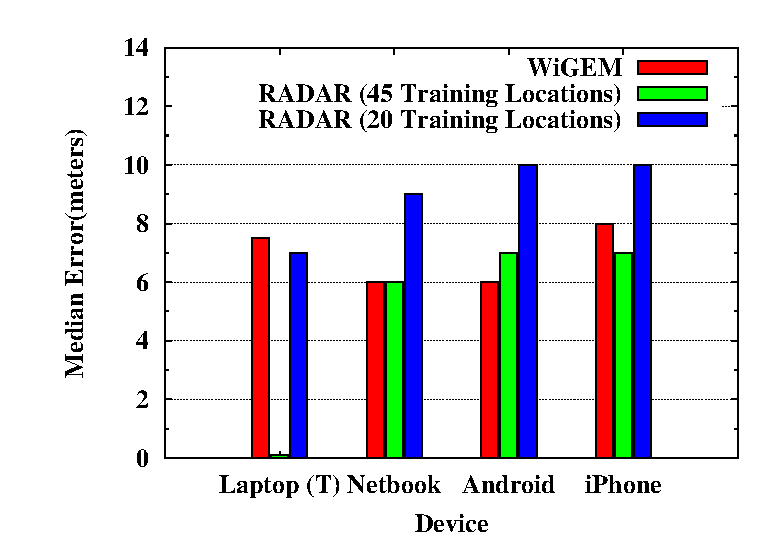
\includegraphics[height=1.5in, width=2.5in]
	      {Figs4Paper/CEWIT/HRComparisons4Paper_CEWIT/HRComparisonsMedianError_RADAR_cewit.eps}}
	\caption{Comparisons on the CEWIT testbed.}
	\label{fig:HR_on_cewittestbed}
\end{figure*}

\begin{figure*}
	\centering
	      \subfloat[WiGEM vs. Probabilistic]{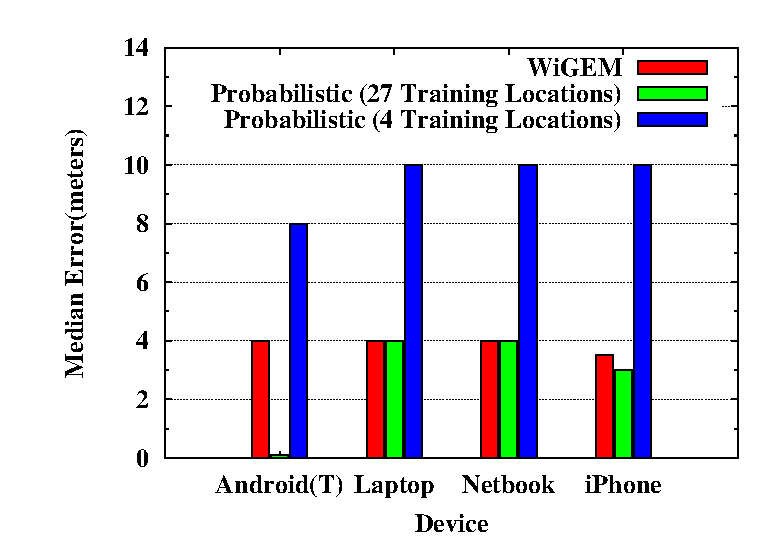
\includegraphics[height=1.5in, width=2.5in]{Figs4Paper/CSD/HRComparisons4Paper_CSD/HRComparisonsMedianError_Probabilistic_csd.eps}}
	      \subfloat[WiGEM vs. RADAR]{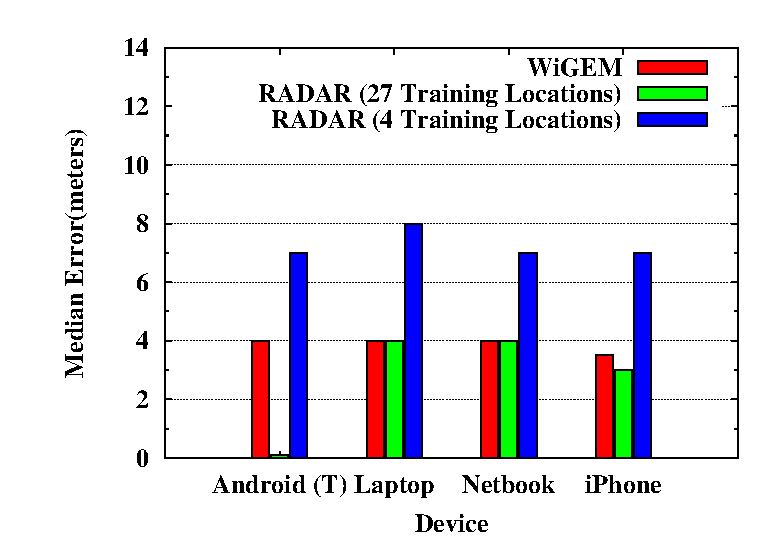
\includegraphics[height=1.5in, width=2.5in]
	      {Figs4Paper/CSD/HRComparisons4Paper_CSD/HRComparisonsMedianError_RADAR_csd.eps}}
	\caption{Comparisons on the CSD testbed.}
	\label{fig:HR_on_csdtestbed}
\end{figure*}

We now compare WiGEM against two popular RF signal map-based schemes that also performed well in literature. We have already reviewed such schemes in Section~\ref{sec:relatedwork}. 
We have picked two representative schemes -- (i) a deterministic scheme, RADAR~\cite{Bahl00radar:an}, that uses the nearest neighbor in signal space (or, an average of $k$
nearest neighbors) as the metric; and (ii) a probabilistic scheme~\cite{Haeberlen:2004:PRL:1023720.1023728, Youssef:2008:HLD:1399551.1399558, Roos} that maintains a probability
distribution of the RSS values from various locations. For the incoming RSS signature, a probability distribution is built over the location space and a location estimate is made. Here, we mainly follow \cite{Haeberlen:2004:PRL:1023720.1023728}, and model RSS as a normal distribution determined by the location and sniffer pair. 

%spend considerable pre-deployment effort in first building an RF signal map from RSS signatures collected from various locations inside the target space. Both schemes differ in the way they handle an incoming signature to provide a location estimate.
%
%\begin{itemize}
%\item Deterministic schemes like RADAR use the nearest neighbor in signal space (or an average of k-nearest neighbors) as the metric to give a location estimate. 
%\item Probabilistic schemes \cite{Haeberlen:2004:PRL:1023720.1023728, Youssef:2008:HLD:1399551.1399558, Roos} on the other hand maintain a probability distribution of the RSS value from various locations. For the incoming signature, a probability distribution is built over the location space and a maximum likelihood estimate is used to determine position. As in \cite{Haeberlen:2004:PRL:1023720.1023728}, we model signal intensity as a normal distribution determined by the location and sniffer pair. 
%\end{itemize}

\subsubsection{Evaluation Setup}
\label{subsubsec:rfsignalmapdiscussion}

%\begin{itemize}

%\item 
For all three techniques we present here, viz., WiGEM, RADAR and Probabilistic, we consider the best location as the location estimate (and not any weighted average of the top few locations). 

%\item
As discussed in Section~\ref{sec:introduction}, the RF map-based techniques need significant `off-line' training and thus are vulnerable to accuracy issues in realistic scenarios as training
and test devices differ. For the CEWIT and CSD testbeds, the Dell laptop 
and the android phone respectively were used for this off-line
training. All four devices were used for testing in all cases. 

%To show the WiFi hardware variance problem mentioned in Section \ref{sec:introduction}, we use different devices for location estimation. For the CEWIT testbed, a DELL Laptop was used to train the radio map during the {\it `offline' phase}. In the CSD testbed, an android phone was used to build the radio map. Based on the radio maps, four different device types are used to give location estimates. 

%\item
Similarly as mentioned in Section~\ref{sec:introduction},
the accuracy of RF map-based techniques depends on the training granularity. 
To evaluate its impact, we consider two scenarios for RADAR and
Probabilistic techniques -- one `optimistic' and the other more `realistic.' In
the optimistic scenario, the training and test data sets are collected at the same physical locations (i.e., 45 and 27 locations in CEWIT and CSD, respectively). In the realistic scenario, the training is done only at a subset 
of the test locations, specifically, 20 and 4 locations in CEWIT and CSD, respectively. 
The testing locations are still uniformly distributed on the grid (Section \ref{subsec:datacollectionmethodology})

%As mentioned in Section \ref{subsec:datacollectionmethodology}, the data for our experimental evaluation is coming from 45 distinct locations on the CEWIT testbed and 27 distinct locations in the CSD testbed. the training and test data sets (mentioned below) are collected at the same physical locations
%
%For RADAR and Probabilistic, we try to understand the effect of the granularity of training locations on the final location estimate. We consider two scenarios : one optimistic and the other more realistic. First, we consider the optimistic secnario where the training and test data sets (mentioned below) are collected at the same physical locations, e.g on the CEWIT testbed, the signal map is built from the same 45 distinct locations where the position estimation is being done. Second, is the more realistic scenario where the training is done from only a subset of the test locations. Thus the testing locations are no longer strictly co-located with the training locations. In the CEWIT testbed, the training is done from 20 locations (out of the 45 possible) roughly every 10.3 meters apart. In the CSD testbed, the subset comprises of 4 locations (out of the 27 possible) roughly every 12.7 meters apart.  We note here that WiGEM on the other hand requires no `pre deployment' training effort. For WiGEM we use the same discretization of the target space that we use in section \ref{subsec:baselinecomparisonwithamodelbasedscheme} i.e the WiGEM location estimate can be on any of the grid points inside the building.

%\item
%There are 200 RSS tuples for every location on the map for each of the four device types. We divide these 200 tuples into two disjoint sets of 100 tuples each. The first set is used by RADAR and Probabilistic to build their RF signal maps while WiGEM uses it as the learning data to build the localization model.  The second set of 100 tuples from each location is used as the test data for all three algorithms. Every device type is evaluated separately. 
%
%\end{itemize}

\begin{figure*}
	\centering
		\subfloat[CEWIT testbed]{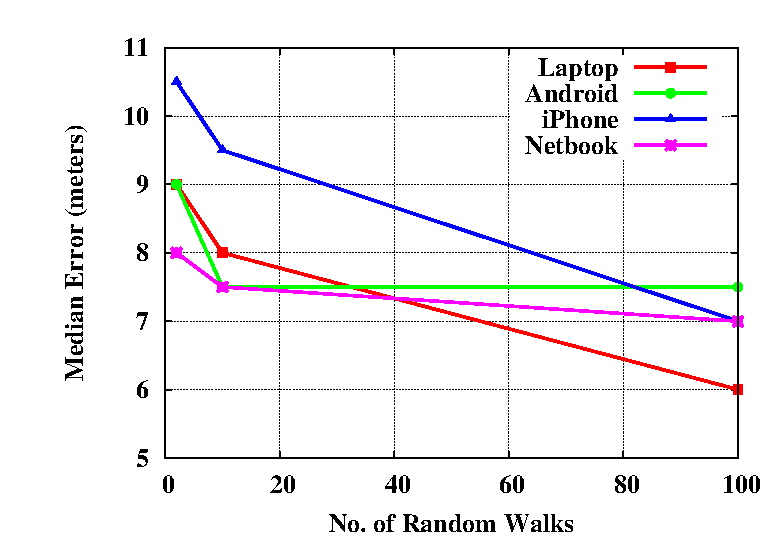
\includegraphics[height=1.5in, width=2.5in]{Figs4Paper/CEWIT/MobilityPlot4paper_CEWIT/Mobility_cewit.eps}}
		\subfloat[CSD testbed]{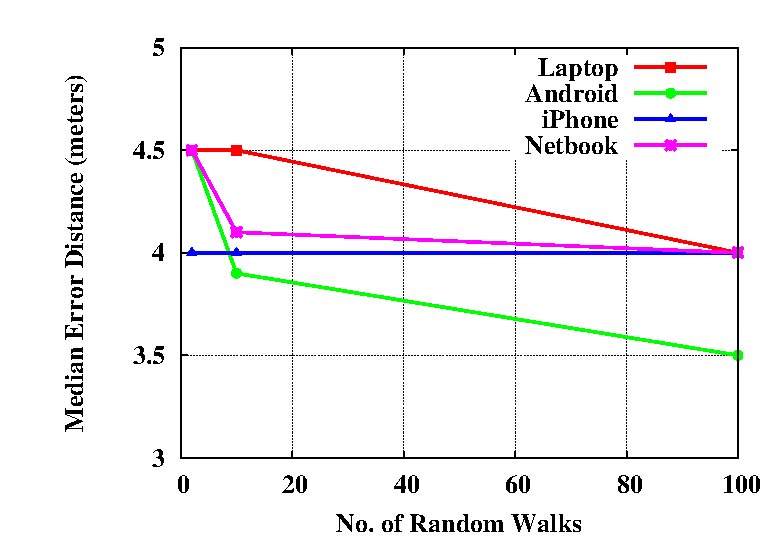
\includegraphics[height=1.5in, width=2.5in]{Figs4Paper/CSD/MobilityPlot4paper_CSD/Mobility_csd.eps}}
	\caption{Impact of mobility during learning for WiGEM.}
	\label{fig:mobility}
\end{figure*}

\subsubsection{Observations}
\label{subsubsec:rfsignalmapobservations}

Figure~\ref{fig:HR_on_cewittestbed} and~\ref{fig:HR_on_csdtestbed} show the median error comparison between the three techniques. We make some interesting observations here.
 
\begin{itemize}

\item 
Hardware variations is a major issue for both RF map based techniques. When the same device is used for training and testing and the same locations are used for training
and testing, the median error is zero. However, when the devices differ
the error jumps up dramatically. This is a critical problem for such techniques, because device hardware will vary widely in a real-world deployment. 

\item
On the other hand, WiGEM cannot match RADAR and Probabilistic for their most 
favorable case (same device, same test locations as training). But it performs
at par with  
RADAR and Probabilistic when devices vary. This is particularly promising because unlike RADAR and Probabilistic, WiGEM does not have the overhead of a pre-deployment training.

\item 
When the granularity of training is coarse, RADAR and Probabilistic show substantially poorer accuracy estimates. Thus, location estimates for such techniques are tightly bound to the granularity of the training effort. WiGEM is almost always better that RADAR and 
Probabilistic when they use coarser grain training. Sometimes the reduction in error
is substantial (more than half). 
%substantially so by reducing the median error by more than half. 
%This makes a stronger case in favor of WiGEM.
%This makes them unattractive for performing localization in large target spaces. A heavy pre-deployment effort also make these techniques difficult to maintain and  update in a dynamic environment.

\end{itemize}

\subsection{Impact of Mobility}
\label{subsec:impactofmobilityongemslocalizationaccuracy}

Finally, we show that the mobility of a client 
does not adversely affect WiGEM's operation or accuracy. In fact, mobility can 
be helpful. The mobility issue is important as for many practical use of
WiGEM (e.g., indoor navigation) the client device can be continuously moving,
providing RSS samples from different locations that may form the learning data set. 

To create the test data set for the mobility evaluation, a user initially walks across all grid locations on the map, making 100 ping transmissions from each location. This forms our test data set which is basically a union of 100 RSS tuples from each location.  Now we  observe the effect of client mobility in localizing this test data set. For the learning part, the user follows a random walk scheme. In each random walk, the user visits every location once, and makes a single ping transmission from that location. This forms the learning data set for WiGEM, in order to build the WiGMM model for the device and provide location estimates for the test data set. 

We evaluate this scheme on both testbeds across four different devices. Figure \ref{fig:mobility} shows how the median localization error for the test data set varies as the mobility (here the number of random walks) increases. Note mobility during learning obviously helps localization. 


